% Preamble
\documentclass[12pt, aspectration=169]{beamer}
\usetheme{Copenhagen}
\usecolortheme{beaver}

\setbeamertemplate{navigation symbols}{}

% Packages
\usepackage{amsmath}
\usepackage{listings}
\usepackage{xcolor}
\usepackage{blkarray}
\usepackage{graphicx}
\usepackage{hyperref}

\definecolor{codegreen}{rgb}{0,0.6,0}
\definecolor{codegray}{rgb}{0.5,0.5,0.5}
\definecolor{codepurple}{rgb}{0.58,0,0.82}
\definecolor{backcolour}{rgb}{0.95,0.95,0.92}

\lstdefinestyle{mystyle}{
    backgroundcolor=\color{backcolour},
    commentstyle=\color{codegreen},
    keywordstyle=\color{magenta},
    numberstyle=\tiny\color{codegray},
    stringstyle=\color{codepurple},
    basicstyle=\ttfamily\footnotesize,
    breakatwhitespace=false,
    breaklines=true,
    captionpos=b,
    keepspaces=true,
    numbers=left,
    numbersep=5pt,
    showspaces=false,
    showstringspaces=false,
    showtabs=false,
    tabsize=4
}

\lstset{style=mystyle}

\title{Introduction to Advanced Python:\\Why is Python slow?}
\author{Kai Striega}
\date{\today}

% Document
\begin{document}

    \maketitle

    \begin{frame}{Before I start}
        \begin{block}{Here be dragons}<2->
            This talk introduces advanced topics, quickly.
            The content is designed to stretch your understanding and to challenge you.
        \end{block}
        \begin{block}{Questions}<3->
            I am happy to take questions during the talk, feel free to ask if something doesn't make sense.
        \end{block}
    \end{frame}

    \begin{frame}{What we're going to do today}
        \begin{itemize}
            \item Answer the question: Why is Python slow?
            \item Compare Python to C
            \item Introduce some of the key ideas in performance analysis
            \item Discuss when execution time matters\ldots and when it doesn't
        \end{itemize}
    \end{frame}

    \begin{frame}{Why C?}
        \begin{columns}
            \column{0.55\textwidth}
            \begin{itemize}
                \item C is \textit{very} fast
                \item C is compiled
                \item CPython is written in C
                \item Many Python extensions are written in C
            \end{itemize}
            \column{0.45\textwidth}
            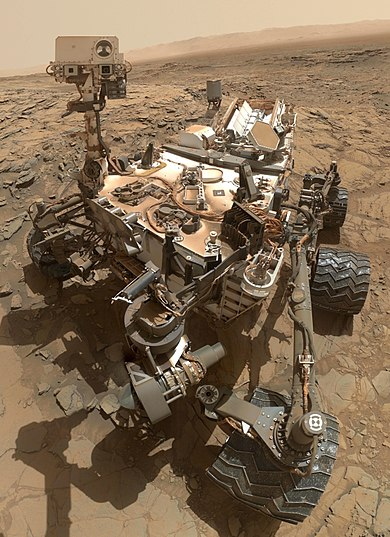
\includegraphics[scale=0.35]{static/images/390px-Curiosity_Self-Portrait_at_'Big_Sky'_Drilling_Site}
        \end{columns}
    \end{frame}

    \begin{frame}{What is a \textit{compiled} language?}
        \begin{center}
            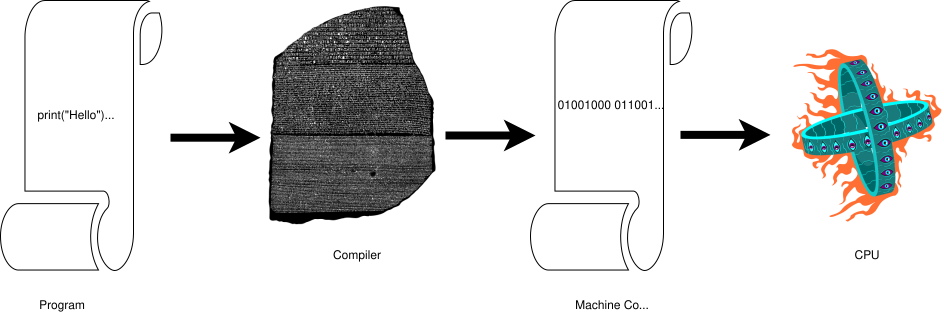
\includegraphics[scale=0.45]{static/images/compiled.drawio}
        \end{center}
    \end{frame}

    \begin{frame}{What the CPU does (Fetch-Execute Cycle)}
        \begin{description}
            \item[Fetch] The CPU fetches the next instruction from the computer's memory based on the value stored in the program counter.
            \item[Decode] The CPU determines what operation needs to be performed and what data (if any) is involved.
            \item[Execute] The CPU performs the operation specified by the instruction.
        \end{description}
    \end{frame}

    \begin{frame}{What limits the performance of the CPU?}
        \begin{description}
            \item[Memory Bound] How quickly we can get data to the CPU
            \item[CPU Bound] How quickly the CPU can execute instructions
        \end{description}
    \end{frame}

    \begin{frame}{Today's Example}
        \lstinputlisting[language=Python,label={lst:python}]{code/sum_of_first_n_numbers.py}
    \end{frame}

    \begin{frame}{Is Python slow?}
        \begin{itemize}
            \item[]<2-> \texttt{time python sum\_of\_first\_n\_numbers.py\newline}
            \item[]<3-> \texttt{total=18446744064889498501\newline
            real 5m56.581s\newline
            user 5m56.518s\newline
            sys 0m0.004s\newline}
        \end{itemize}
    \end{frame}

    \begin{frame}{Today's Example, but in C}
        \lstinputlisting[language=C,label={lst:C}]{code/sum_of_first_n_numbers.c}
    \end{frame}

    \begin{frame}{What about C?}
        \begin{itemize}
            \item[]<2-> \texttt{time bin/sum\_of\_first\_n\_numbers\_O3\newline}
            \item[]<3-> \texttt{total=18446744064889498501\newline
            real 0m0.000s\newline
            user 0m0.000s\newline
            sys 0m0.000s\newline}
        \end{itemize}
    \end{frame}

    \begin{frame}{Why?}
        \begin{itemize}
            \item \textit{0m0.000s} seems like a bug\ldots it's not!
            \item C is a \textbf{compiled} langauge
            \item The compiler can perform optimizations on the code
        \end{itemize}
    \end{frame}

    \begin{frame}{Optimising Compilers}
        \begin{itemize}
            \item Our problem is always going to have the same answer
            \item The compiler is able to notice this
            \item And calculates the result ahead of time
            \item So how do we get around this?
        \end{itemize}
    \end{frame}

    \begin{frame}{What if we don't use optimizations?}
        \begin{itemize}
            \item[]<2-> \texttt{time bin/sum\_of\_first\_n\_numbers\_arg\_O0\newline}
            \item[]<3-> \texttt{total=18446744064889498501\newline
            real 0m2.020s\newline
            user 0m2.010s\newline
            sys 0m0.010s\newline}
        \end{itemize}
    \end{frame}

    \begin{frame}{What we've done so far}
        \begin{itemize}
            \item We've turned a 6-minute problem into a 2-second problem
            \item By changing the language
            \item This speedup exists even without optimizations
        \end{itemize}
    \end{frame}

    \begin{frame}{What makes C so much faster than Python?}
        \begin{description}
            \item[Interpreted vs Compiled] Python is \textit{interpreted} $\implies$ CPU has to do extra work to translate the code at runtime
            \item[Memroy Access Patterns] Python stores everything in a \textit{PyObject} this means the CPU can't access data as efficiently
        \end{description}
        Both interpreting code and memory access patterns are limited by the CPU.
    \end{frame}

    \begin{frame}{What does it take to interpet Python?}
        \begin{description}
            \item[Source Code] You start with a Python source code file (typically ending in .py) that contains the instructions you want the computer to execute.
            \item[Tokenizer] The source code is read by the Python interpreter, which breaks it down into a series of tokens.
            \item[Parser] This is where the interpreter checks if the arrangement of tokens conforms to the rules of the Python language.
        \end{description}
    \end{frame}

    \begin{frame}{What does it take to interpet Python?}
        \begin{description}
            \item[AST] An \textit{abstract syntax tree} is a hierarchical representation of the program's structure.
            The nodes of the tree represent operations, while the edges represent control flow.
            \item[Semantic Analysis] The interpreter now checks the AST for semantic correctness.
            \item[Execution] The Python interpreter executes the code by walking through the AST and performing the operations specified by the source code.
        \end{description}
    \end{frame}

    \begin{frame}{Memory Latencies}
        \begin{center}
            \begin{tabular}{|c c|}
             \hline
              & Latency \\ [0.5ex]
             \hline\hline
             L1 Cache & $<$1ns \\
             \hline
             L2 Cache & 4ns \\
             \hline
             Main Memory & 100ns \\
             \hline
             SSD & 16 $\mu$s \\ [1ex]
             \hline
             Round Trip (Datacenter)   & 0.5ms     \\
             \hline
             Round Trip (US to Europe) & 150 ms \\ [1ex]
             \hline
            \end{tabular}
        \end{center}
    \end{frame}

    \begin{frame}{Memory Latencies}
        \begin{center}
            \begin{tabular}{|c c|}
             \hline
              & Latency \\ [0.5ex]
             \hline\hline
             L1 Cache & $<$1 second \\
             \hline
             L2 Cache & 4 seconds \\
             \hline
             Main Memory & 100 seconds \\
             \hline
             SSD & 4.5 hours \\ [1ex]
             \hline
             Round Trip (Datacenter)   & 5.8 days     \\
             \hline
             Round Trip (US to Europe) & 5 years \\ [1ex]
             \hline
            \end{tabular}
        \end{center}
    \end{frame}

    \begin{frame}{Performance Considerations}
        \begin{itemize}
            \item Want to get data from the \textit{fastest} possible source
            \item Usually that will be a \textit{cache} or \textit{memory} (RAM)
            \item Want to avoid network access as much as possible
        \end{itemize}
    \end{frame}

    \begin{frame}{What is a PyObject?}
        \begin{itemize}
            \item Everything in Python is an \textit{Object}
            \item An object is represented as a \textit{PyObject} in C code
            \item You can think of a PyObject as a wrapper around the data and some metadata
        \end{itemize}
    \end{frame}

    \begin{frame}{A Python int is more than a C int}
        \begin{itemize}
            \item[] \begin{center}
                  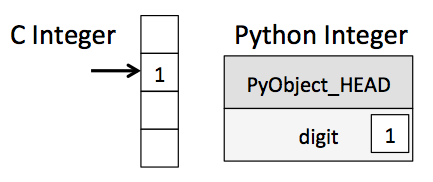
\includegraphics[scale=0.5]{static/images/cint_vs_pyint}
            \end{center}
        \end{itemize}
    \end{frame}

    \begin{frame}{This extends to more complex data structures}
        \begin{center}
              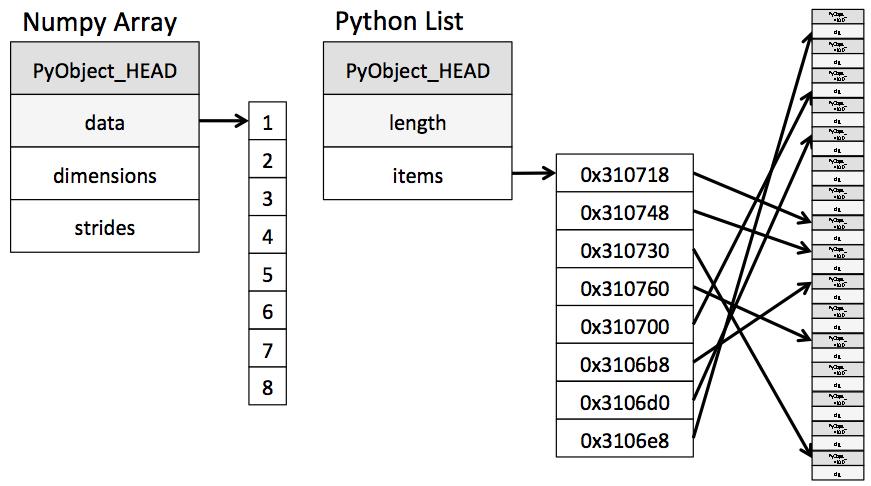
\includegraphics[scale=0.25]{static/images/array_vs_list}
        \end{center}
    \end{frame}

    \begin{frame}{Python's slowness doesn't matter}
        \begin{itemize}
            \item The number of problems where Python is \textit{truly} the bottleneck is very small
            \item Developers are expensive, Python is quick to develop with
            \item Many problems can be solved by throwing more hardware at them (horizontally scalable)
            \item Many problems are bound by network time, not CPU time
        \end{itemize}
    \end{frame}

    \begin{frame}{Further Reading}
        \begin{itemize}
            \item \url{https://www.oreilly.com/library/view/high-performance-python/9781492055013/}
            \item \url{https://www.amazon.com.au/Architecture-Departments-Electrical-Engineering-University-dp-0128119055/dp/0128119055/ref=dp_ob_title_bk}
            \item \url{https://www.oreilly.com/library/view/designing-data-intensive-applications/9781491903063/}
        \end{itemize}
        \begin{center}
            \begin{columns}
                \column{0.30\textwidth}
                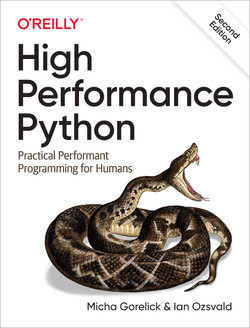
\includegraphics[scale=0.35]{static/images/HighPerformancePython2ndEdition}
                \column{0.30\textwidth}
                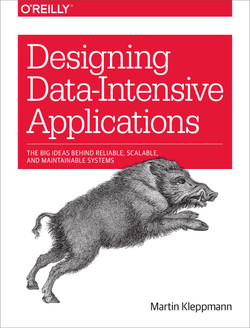
\includegraphics[scale=0.35]{static/images/designing_data_intensive_applications}
                \column{0.30\textwidth}
                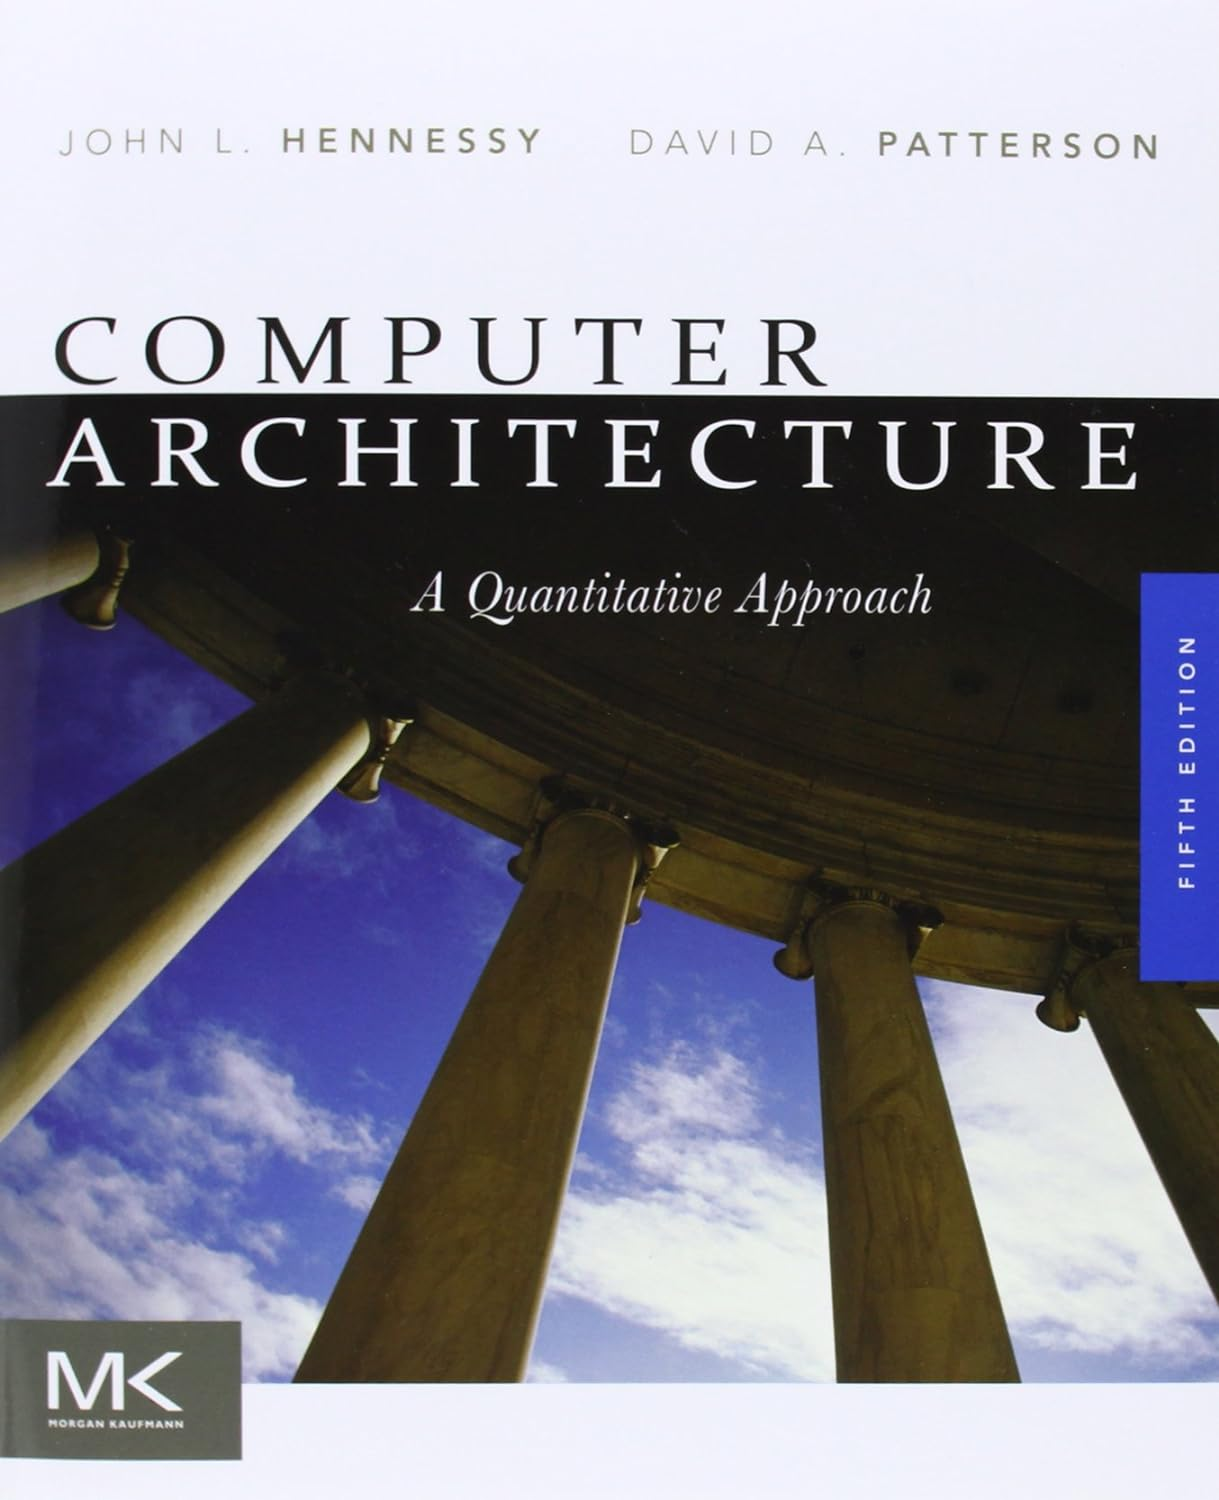
\includegraphics[scale=0.075]{static/images/computer_architecture}
            \end{columns}
        \end{center}
    \end{frame}

\end{document}